\chapter{注意力机制}
\label{ch:attention}

注意力机制是现代深度学习(尤其是 Transformer 模型)的灵魂,它允许模型动态地关注输入序列的不同部分。

\section{缩放点积注意力 (Scaled Dot-Product Attention)}

\begin{variable}
\begin{itemize}
    \item $Q \in \mathbb{R}^{N \times d_k}$: 查询矩阵 (Query),$N$ 为序列长度。
    \item $K \in \mathbb{R}^{M \times d_k}$: 键矩阵 (Key),$M$ 为 Context 长度。
    \item $V \in \mathbb{R}^{M \times d_v}$: 值矩阵 (Value)。
    \item $d_k$: 键向量的维度,用于缩放因子 $\sqrt{d_k}$。
\end{itemize}
\end{variable}

\begin{figure}[h]
    \centering
    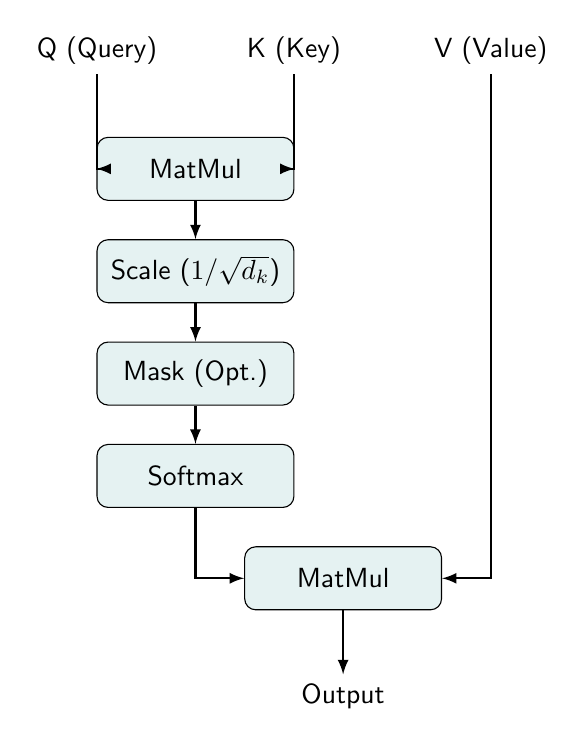
\begin{tikzpicture}[
        op/.style={draw, rectangle, rounded corners, fill=teal!10, minimum width=2.5cm, minimum height=0.8cm, align=center, font=\sffamily},
        data/.style={font=\sffamily},
        arrow/.style={-latex, thick}
    ]
        
        % Data inputs (Absolute positioning)
        \node[data] (q) at (0, 0) {Q (Query)};
        \node[data] (k) at (2.5, 0) {K (Key)};
        \node[data] (v) at (5, 0) {V (Value)};
        
        % Operations (Absolute positioning)
        \node[op] (matmul1) at (1.25, -1.5) {MatMul};
        \node[op] (scale) at (1.25, -2.8) {Scale ($1/\sqrt{d_k}$)};
        \node[op] (mask) at (1.25, -4.1) {Mask (Opt.)};
        \node[op] (softmax) at (1.25, -5.4) {Softmax};
        \node[op] (matmul2) at (3.125, -6.7) {MatMul};
        
        % Output
        \node[data] (out) at (3.125, -8.2) {Output};
        
        % Arrows
        \draw[arrow] (q) |- (matmul1);
        \draw[arrow] (k) |- (matmul1);
        \draw[arrow] (matmul1) -- (scale);
        \draw[arrow] (scale) -- (mask);
        \draw[arrow] (mask) -- (softmax);
        \draw[arrow] (softmax) |- (matmul2);
        \draw[arrow] (v) |- (matmul2);
        \draw[arrow] (matmul2) -- (out);
        
    \end{tikzpicture}
    \caption{缩放点积注意力的数据流图 (Scaled Dot-Product Attention)}
    \label{fig:attention}
\end{figure}

\begin{rosetta}{Self-Attention}
    \begin{equation}
        \text{Attention}(Q, K, V) = \text{softmax}\left(\frac{QK^T}{\sqrt{d_k}}\right)V
    \end{equation}
    其中:
    \begin{itemize}
        \item $Q$ (Query), $K$ (Key), $V$ (Value) 是线性变换后的矩阵。
        \item $d_k$ 是 Key 的维度,除以 $\sqrt{d_k}$ 是为了防止点积结果过大导致梯度消失。
    \end{itemize}
    \tcblower
    \pyfunc{torch.nn.functional.scaled\_dot\_product\_attention}
\end{rosetta}

\section{多头注意力 (Multi-Head Attention)}

多头注意力通过并行运行多个自注意力头,使模型能够同时从不同的表示子空间捕捉信息。

\begin{center}
\begin{tikzpicture}[node distance=1.2cm, font=\sffamily\small]
    % 输入
    \node[data_node] (in) {Input $X$};
    
    % 线型投影
    \node[block, above=0.8cm of in] (proj) {Linear Projections \\ ($W^Q_i, W^K_i, W^V_i$)};
    \draw[conn] (in) -- (proj);
    
    % 多头并行
    \node[attn_block, above left=1cm and 0.5cm of proj] (h1) {Scaled Dot-Product \\ Head 1};
    \node[attn_block, above right=1cm and 0.5cm of proj] (h2) {Scaled Dot-Product \\ Head 2};
    \node[above=0.8cm of proj] (dots) {$\dots$};
    
    \draw[conn] (proj.north) -- (h1.south);
    \draw[conn] (proj.north) -- (h2.south);
    
    % 拼接
    \node[block, above=3cm of proj] (concat) {Concatenation};
    \draw[conn] (h1.north) -- (concat.west);
    \draw[conn] (h2.north) -- (concat.east);
    
    % 输出投影
    \node[block, above=0.8cm of concat] (out_proj) {Linear $W^O$};
    \draw[conn] (concat) -- (out_proj);
    \node[above=0.6cm of out_proj] (out) {Output};
    \draw[conn] (out_proj) -- (out);

    % 背景容器
    \begin{scope}[on background layer]
        \node[container, fit=(h1) (h2) (dots)] (heads_box) {};
        \node[anchor=north east, brandblue!50] at (heads_box.north east) {Multi-Heads};
    \end{scope}
\end{tikzpicture}
\end{center}

\begin{rosetta}{多头注意力计算}
    \begin{equation}
        \text{MultiHead}(Q, K, V) = \text{Concat}(\text{head}_1, \dots, \text{head}_h)W^O
    \end{equation}
    其中 $\text{head}_i = \text{Attention}(QW_i^Q, KW_i^K, VW_i^V)$
    \tcblower
    \pyfunc{nn.MultiheadAttention(embed\_dim, num\_heads)}
\end{rosetta}
